\documentclass{article}
\usepackage[spanish]{babel}
\usepackage[letterpaper,top=2cm,bottom=2cm,left=3cm,right=3cm,marginparwidth=1.75cm]{geometry}
\usepackage{graphicx}
\usepackage{listings}
\usepackage{color}
\usepackage{hyperref}

\definecolor{mygray}{rgb}{0.5,0.5,0.5}
\definecolor{mymauve}{rgb}{0.58,0,0.82}

\lstset{
	language=SQL,
	numbers=left,
	stepnumber=1,
	numbersep=8pt,
	showspaces=false,
	showstringspaces=false,
	showtabs=false,
	frame=lines,
	rulecolor=\color{black},
	tabsize=2,
	breaklines=true,
	breakatwhitespace=false,
	title=\lstname,
	keywordstyle=\color{blue},
	commentstyle=\color{mygray},
	stringstyle=\color{mymauve},
	captionpos=b,
	escapeinside={\%*}{*)},
	morekeywords={*,REPLACE}
}
\graphicspath{ {./images/} }


\title{Formula 1}
\author{Farid Marcos Bustos Casij - 20022114011\\ Rafael Ortiz Reales -  2023114117}


\begin{document}
	\maketitle
	\section{Historias de usuario}
	\subsection*{Estructura}
		\begin{itemize}
			
			\item \large{\textbf{Enunciado}}
			\begin{description}
				Como [tipo de usuario], quiero [una acción] para [beneficio/valor]
			\end{description}
			
			\item \large{\textbf{Descripción}}
			\begin{description}
				[Tipo de usuario] debe estar en la capacidad de [una acción]. Se deben incluir todos los detalles clave [Detalles]
			\end{description}
			
			\item \large{\textbf{Criterios de aceptación}}
			\begin{itemize}
				\item Criterio de aceptación
			\end{itemize}
			
		\end{itemize}
		
	\subsection{Historia 1}
		\begin{itemize}
			
			\item \large{\textbf{Enunciado}}
			\begin{description}
				Como administrador de eventos de la Fórmula 1, quiero poder almacenar la información de todos los equipos que alguna vez han participado en cualquier competencia de la Fórmula 1 para llevar una cuenta de cuántos equipos diferentes han existido a lo largo de la historia de la Fórmula 1.
			\end{description}
			
			\item \large{\textbf{Descripción}}
			\begin{description}
				El administrador debe tener la capacidad de registrar información detallada de los equipos que alguna vez han participado en cualquier temporada a lo largo de la historia de la Fórmula 1. Esto incluye el nombre del equipo, país de origen, nombres de los directores del equipo, años de participación y otros datos relevantes.
				
			\end{description}
			
			\item \large{\textbf{Criterios de aceptación}}
			\begin{itemize}
				\item Debe ser posible registrar el nombre del equipo.
				\item Debe ser posible registrar el país de origen del equipo.
				\item Debe ser posible registrar los nombres de los directores del equipo. 
				\item Debe ser posible registrar el las temporadas en las que participa cada equipo.
			\end{itemize}
			
		\end{itemize}
	
	\subsection{Historia 2}
	\begin{itemize}
		
		\item \large{\textbf{Enunciado}}
		\begin{description}
			Como administrador de eventos de la Fórmula 1, quiero poder almacenar la información de las personas que conforman un equipo de la Fórmula 1 para así poder facilitar así la organización y la comunicación interna durante el desarrollo y ejecución de eventos de la Fórmula 1.
		\end{description}
		
		\item \large{\textbf{Descripción}}
		\begin{description}
			El administrador debe tener la capacidad de registrar información de los miembros del equipo de la Fórmula 1. Esto incluye nombres, roles dentro del equipo, datos de contacto y cualquier otra información relevante
		\end{description}
		
		\item \large{\textbf{Criterios de aceptación}}
		\begin{itemize}
			\item Debe ser posible registrar los nombres de cada miembro del equipo.
			\item Debe ser posible registrar los roles de cada miembro del equipo.
			\item Debe ser posible ingresar datos de contacto como correo electrónico y número de teléfono.
		\end{itemize}
		
	\end{itemize}
	
	\subsection{Historia 3}
	\begin{itemize}
		
		\item \large{\textbf{Enunciado}}
		\begin{description}
			Como administrador de eventos de la Fórmula 1, quiero poder almacenar la información de los patrocinadores de los equipos de Fórmula 1 para verificar que se haga cumplimiento de las normativas establecidas en cuanto al dinero máximo que se puede recibir de los patrocinios.
			
		\end{description}
		
		\item \large{\textbf{Descripción}}
		\begin{description}
			El administrador debe poder registrar información de los patrocinadores de cada equipo de la Fórmula 1. Esto incluye el nombre del patrocinador, monto patrocinado y la relación con el equipo.

		\end{description}
		
		\item \large{\textbf{Criterios de aceptación}}
		\begin{itemize}
			\item Debe ser posible registrar el nombre del patrocinador.
			
			\item Debe ser posible registrar la cantidad de dinero que un patrocinador le da a un equipo.
			
			\item Debe ser posible registrar los equipos que patrocina.
			
			\item Debe ser posible registrar la duración del patrocinio.
			
			\item Debe ser posible registrar si el patrocinio es exclusivo o no.
			
		\end{itemize}
		
	\end{itemize}
	
	\subsection{Historia 4}
	\begin{itemize}
		
		\item \large{\textbf{Enunciado}}
		\begin{description}
			Como administrador de eventos de la Fórmula 1, quiero poder almacenar la información de los equipos que participaran en una temporada de la fórmula 1 para facilitar la planificación y coordinación logística de los eventos de la temporada de la Fórmula 1.
			
		\end{description}
		
		\item \large{\textbf{Descripción}}
		\begin{description}
			El administrador debe tener la capacidad de registrar los equipos que participarán en una temporada específica de la Fórmula 1. Esto incluye el nombre del equipo, país de origen y cualquier otro dato relevante para la logística
			
		\end{description}
		
		\item \large{\textbf{Criterios de aceptación}}
		\begin{itemize}
			\item Debe ser posible registrar el equipo que participara.
			\item Debe ser posible registrar la temporada en la que participa.
			
		\end{itemize}
		
	\end{itemize}
	
	\subsection{Historia 5}
	\begin{itemize}
		
		\item \large{\textbf{Enunciado}}
		\begin{description}
Como administrador de eventos de la Fórmula 1, quiero poder almacenar la información de los grandes premios que se llevan a cabo dentro de una temporada para poder consultarlos cuando sea necesario y mantener informados a los fanáticos de la Fórmula 1.
		\end{description}
		
		\item \large{\textbf{Descripción}}
		\begin{description}
	El administrador debe poder registrar información sobre los grandes premios de cada temporada. Esto incluye el nombre del gran premio, ubicación, fecha y cualquier otro dato relevante.

		\end{description}
		
		\item \large{\textbf{Criterios de aceptación}}
		\begin{itemize}
			\item Debe ser posible registrar el nombre del gran premio.
			\item Debe ser posible registrar la ciudad en la que se llevará a cabo  el gran premio. 
			\item Debe ser posible registrar el circuito que se utilizara. 
			\item Debe ser posible registrar la fecha de inicio del evento. 
			\item Debe ser posible registrar la fecha de finalizacion del evento.
			
		\end{itemize}
		
	\end{itemize}
	
	\subsection{Historia 6}
	\begin{itemize}
		
		\item \large{\textbf{Enunciado}}
		\begin{description}
			Como administrador de eventos de la fórmula 1, quiero poder almacenar la información de los circuitos que se pueden utilizar para llevar a cabo eventos de la fórmula 1 para poder planear en donde se llevarán a cabo los grandes premios de la fórmula 1.
			
		\end{description}
		
		\item \large{\textbf{Descripción}}
		\begin{description}
			El administrador debe poder registrar información de los circuitos disponibles para los eventos de la Fórmula 1. Esto incluye el nombre del circuito, ubicación, longitud y cualquier otra información relevante. 
			
		\end{description}
		
		\item \large{\textbf{Criterios de aceptación}}
		\begin{itemize}
			\item Debe ser posible registrar el nombre del circuito
			\item Debe ser posible registrar la ciudad en la que se encuentra el circuito.
			\item Debe ser posible ingresar la longitud del circuito. 
			
		\end{itemize}
		
	\end{itemize}
	
	\subsection{Historia 7}
	\begin{itemize}
		
		\item \large{\textbf{Enunciado}}
		\begin{description}
			Como administrador de eventos de la Fórmula 1, quiero poder almacenar la información de las carreras que se realizan para poder mantener informados a los fanáticos de la Fórmula 1.
			
		\end{description}
		
		\item \large{\textbf{Descripción}}
		\begin{description}
			El administrador debe poder registrar información de todas las carreras realizadas en una temporada de la Fórmula 1. Esto incluye la fecha, ubicación, equipos participantes y resultados. 
			
		\end{description}
		
		\item \large{\textbf{Criterios de aceptación}}
		\begin{itemize}
			\item Debe ser posible registrar la fecha de cada carrera.
			\item Debe ser posible registrar la hora de cada carrera.
			\item Debe ser posible registrar el circuito de cada carrera. 
			\item Debe ser posible registrar los equipos que participan.
			\item Debe ser posible registrar los pilotos que participan
			\item Debe ser posible registrar qué tipo de carrera es. 
			
		\end{itemize}
		
	\end{itemize}
	
	\subsection{Historia 8}
	\begin{itemize}
		
		\item \large{\textbf{Enunciado}}
		\begin{description}
Como administrador de eventos de la Fórmula 1, quiero poder almacenar la información de los vehículos que posee cada equipo para facilitar el manejo de los recursos de la competición.

		\end{description}
		
		\item \large{\textbf{Descripción}}
		\begin{description}
El administrador debe poder registrar información detallada de los vehículos que cada equipo posee. Esto incluye el modelo del vehículo, especificaciones técnicas y el equipo al que pertenece. 

		\end{description}
		
		\item \large{\textbf{Criterios de aceptación}}
		\begin{itemize}
			\item Debe ser posible registrar el tipo de motor de cada vehículo. 
			\item Debe ser posible registrar el tipo de neumático de cada vehículo. 
			\item Debe ser posible registrar a que equipo le pertenece cada vehículo. 
			
		\end{itemize}
		
	\end{itemize}
	
	\subsection{Historia 9}
	\begin{itemize}
		
		\item \large{\textbf{Enunciado}}
		\begin{description}
Como administrador de eventos de la Fórmula 1, quiero poder almacenar la información de los vehículos que utilizan los pilotos en una carrera para hacer mejores planes de logística al organizar las carreras.
		\end{description}
		
		\item \large{\textbf{Descripción}}
		\begin{description}
El administrador debe poder registrar información de los vehículos utilizados por cada piloto en una carrera específica. Esto incluye el modelo del vehículo, el piloto que lo utiliza y la carrera correspondiente. 

		\end{description}
		
		\item \large{\textbf{Criterios de aceptación}}
		\begin{itemize}
			\item Debe ser posible registrar las carreras en las que se utiliza el vehículo.
			\item Debe ser posible registrar los pilotos que utilizan el vehículo en una carrera.
			\item Debe ser posible registrar el vehículo utilizado.
			
		\end{itemize}
		
	\end{itemize}
	
	\subsection{Historia 10}
	\begin{itemize}
		
		\item \large{\textbf{Enunciado}}
		\begin{description}
		Como administrador de eventos de la Fórmula 1, quiero poder almacenar la información de los accidentes que ocurren en una carrera para facilitar un registro detallado y preciso de los siniestros que ocurran durante una carrera.
		\end{description}
		
		\item \large{\textbf{Descripción}}
		\begin{description}
		El administrador debe poder registrar información detallada sobre los accidentes que ocurren durante una carrera. Esto incluye el piloto involucrado, el vehículo, la naturaleza del accidente y las consecuencias. 

		\end{description}
		
		\item \large{\textbf{Criterios de aceptación}}
		\begin{itemize}
			\item Debe ser posible registrar el piloto involucrado en el accidente.
			\item Debe ser posible registrar el vehículo involucrado en el accidente. 
			\item Debe ser posible registrar detalles sobre la naturaleza y causas del accidente. 
			\item Debe ser posible registrar las consecuencias del accidente.
			
		\end{itemize}
		
	\end{itemize}
	
	\subsection{Historia 11}
	\begin{itemize}
		
		\item \large{\textbf{Enunciado}}
		\begin{description}
			Como administrador de eventos de la Fórmula 1, quiero poder almacenar la información de las sanciones que se les hace a los pilotos en una carrera para facilitar un seguimiento detallado de las sanciones impuestas a los pilotos durante una carrera.
			
		\end{description}
		
		\item \large{\textbf{Descripción}}
		\begin{description}
			El administrador debe poder registrar información sobre las sanciones impuestas a los pilotos durante una carrera. Esto incluye el piloto sancionado, la razón de la sanción, el tipo de sanción y la carrera correspondiente. 
			
		\end{description}
		
		\item \large{\textbf{Criterios de aceptación}}
		\begin{itemize}
			\item Debe ser posible registrar el piloto sancionado.
			\item Debe ser posible registrar la razón de la sanción.
			\item Debe ser posible registrar la penalización de la sanción. 
			\item Debe ser posible registrar la vuelta en la que ocurrió dicha sanción.
			
		\end{itemize}
		
	\end{itemize}
	
	\subsection{Historia 12}
	\begin{itemize}
		
		\item \large{\textbf{Enunciado}}
		\begin{description}
			Como administrador de eventos de la Fórmula 1, quiero poder almacenar la información de las paradas en los Boxes que hacen los pilotos en una carrera para facilitar el seguimiento y la gestión eficiente de las paradas en boxes realizadas por los pilotos durante una carrera.
			
		\end{description}
		
		\item \large{\textbf{Descripción}}
		\begin{description}
			El administrador debe poder registrar información sobre las paradas en los PIT realizadas por los pilotos durante una carrera. Esto incluye el piloto, el vehículo, el tiempo de parada, y los servicios realizados durante la parada.
			
		\end{description}
		
		\item \large{\textbf{Criterios de aceptación}}
		\begin{itemize}
			\item Debe ser posible registrar el piloto que realiza la parada.
			\item Debe ser posible registrar el vehículo que realiza la parada. 
			\item Debe ser posible registrar la duración de la parada.
			\item Debe ser posible registrar los servicios realizados (como cambio de llantas, repostaje, etc.).
			
		\end{itemize}
		
	\end{itemize}
	
	\subsection{Historia 13}
	\begin{itemize}
		
		\item \large{\textbf{Enunciado}}
		\begin{description}
			Como administrador de eventos de la Fórmula 1, quiero poder almacenar cada una de las temporadas de la Fórmula 1 para así llevar un historial de los equipos, carreras y patrocinadores que estuvieron presentes en una temporada en específico.
			
		\end{description}
		
		\item \large{\textbf{Descripción}}
		\begin{description}
			El administrador debe poder registrar, actualizar las temporadas disponibles en la base de datos, así como la información relacionada con los equipos, carreras y patrocinadores de cada temporada.
			
		\end{description}
		
		\item \large{\textbf{Criterios de aceptación}}
		\begin{itemize}
			\item Debe ser posible registrar la fecha de inicio de la temporada.
			\item Debe ser posible registrar la fecha de finalización de la temporada.
			\item Debe ser posible registrar el número de grandes premios que toman lugar \item en una temporada.
			
		\end{itemize}
		
	\end{itemize}
	
	\subsection{Historia 14}
	\begin{itemize}
		
		\item \large{\textbf{Enunciado}}
		\begin{description}
Como administrador de eventos de la Fórmula 1, quiero poder almacenar la información de los motores que podrían utilizar los vehículos en una competencia para que los equipos tengan más control sobre las especificaciones de sus vehículos.

		\end{description}
		
		\item \large{\textbf{Descripción}}
		\begin{description}
El administrador debe poder registrar información sobre los motores permitidos en las competiciones de la Fórmula 1. 

		\end{description}
		
		\item \large{\textbf{Criterios de aceptación}}
		\begin{itemize}
			\item Debe ser posible registrar la marca
			\item Debe ser posible registrar el número de válvulas
			\item Debe ser posible registrar el tipo de motor
			\item Debe ser posible registrar el modelo
			\item Debe ser posible registrar el material del cigüeñal
			\item Debe ser posible registrar el material del árbol de levas
			
		\end{itemize}
		
	\end{itemize}
	
	\subsection{Historia 15}
	\begin{itemize}
		
		\item \large{\textbf{Enunciado}}
		\begin{description}
Como administrador de eventos de la Fórmula 1, quiero poder almacenar la información de los tipos de llantas que pueden utilizar los vehículos en una competencia para que los equipos conozcan cómo pueden diseñar los vehículos y evitar sanciones.

		\end{description}
		
		\item \large{\textbf{Descripción}}
		\begin{description}
El administrador debe poder registrar información sobre los tipos de llantas permitidas en las competiciones de la Fórmula 1.

		\end{description}
		
		\item \large{\textbf{Criterios de aceptación}}
		\begin{itemize}
			\item Debe ser posible registrar la dureza de las llantas.
			\item Debe ser posible registrar los vehículos que utilizan los tipos de llantas.
			
		\end{itemize}
		
	\end{itemize}
	
	\subsection{Historia 16}
	\begin{itemize}
		
		\item \large{\textbf{Enunciado}}
		\begin{description}
			Como administrador de eventos de la Fórmula 1, quiero poder almacenar la información de los puntajes que se reciben al terminar en una posición en específico en una carrera para facilitar el cálculo y seguimiento precisos de los puntajes otorgados a los pilotos en función de su posición final en cada carrera.

		\end{description}
		
		\item \large{\textbf{Descripción}}
		\begin{description}
			El administrador debe poder registrar el sistema de puntuación utilizado en las competiciones de la Fórmula 1. Esto incluye los puntos asignados a cada posición final en las carreras y las reglas para la asignación de estos puntos.

		\end{description}
		
		\item \large{\textbf{Criterios de aceptación}}
		\begin{itemize}
			\item Debe ser posible registrar la posición del puntaje.
			\item Debe ser posible registrar los puntajes otorgados a cada posición.
			
		\end{itemize}
		
	\end{itemize}
	
	\subsection{Historia 17}
	\begin{itemize}
		
		\item \large{\textbf{Enunciado}}
		\begin{description}
			Como administrador de eventos de la Fórmula 1, quiero poder almacenar los tiempos de las vueltas más rápidas realizadas por cada piloto durante una carrera, para destacar los logros individuales y comparar el rendimiento entre pilotos y equipos.

		\end{description}
		
		\item \large{\textbf{Descripción}}
		\begin{description}
			El administrador debe poder registrar los tiempos de las vueltas más rápidas realizadas por los pilotos en cada carrera. Esto incluye el tiempo de la vuelta, el piloto, el equipo, y la carrera correspondiente.

		\end{description}
		
		\item \large{\textbf{Criterios de aceptación}}
		\begin{itemize}
			\item Debe ser posible registrar el tiempo de la vuelta más rápida realizada por cada piloto. 
			\item Debe ser posible registrar la carrera en la que hizo esa vuelta.
			\item Debe ser posible registrar el vehículo que utilizó el piloto durante la vuelta.
			
		\end{itemize}
		
	\end{itemize}
	
	\subsection{Historia 18}
	\begin{itemize}
		
		\item \large{\textbf{Enunciado}}
		\begin{description}
			Como analista de marketing de la Fórmula 1, quiero poder almacenar datos actualizados sobre la asistencia a las carreras, las audiencias y las cifras de streaming en línea para cada carrera, para  evaluar el alcance y el impacto de nuestra marca.
			
		\end{description}
		
		\item \large{\textbf{Descripción}}
		\begin{description}
		El analista de marketing debe estar en la capacidad de almacenar datos sobre la cantidad de persona que ve una carrera así como también la plataforma donde la ven. Se deben incluir detalles clave como audiencia y plataforma de streaming.
		\end{description}
		
		\item \large{\textbf{Criterios de aceptación}}
		\begin{itemize}
			\item Se debe poder almacenar la audiencia
			\item Se debe poder almacenar la plataforma de streaming.
		\end{itemize}
		
	\end{itemize}
	
	\subsection{Historia 19}
	\begin{itemize}
		
		\item \large{\textbf{Enunciado}}
		\begin{description}
		Como administrador de eventos de la Fórmula 1, quiero poder almacenar noticias y comunicados de prensa relacionados con la Fórmula 1, para mantener un registro actualizado de la cobertura mediática y poder acceder a información relevante sobre eventos, pilotos, equipos y decisiones importantes.

		\end{description}
		
		\item \large{\textbf{Descripción}}
		\begin{description}
El administrador debe poder registrar noticias y comunicados de prensa relacionados con la Fórmula 1. 

		\end{description}
		
		\item \large{\textbf{Criterios de aceptación}}
		\begin{itemize}
			\item Debe ser posible registrar la fecha de publicación de la noticia.
			\item Debe ser posible registrar la hora de publicación de la noticia.
			\item Debe ser posible registrar el contenido de cada noticia o comunicado.
			\item Debe ser posible registrar el título de cada noticia o comunicado. 
			\item Debe ser posible registrar el autor de cada noticia
			
		\end{itemize}
		
	\end{itemize}
	
	\subsection{Historia 20}
	\begin{itemize}
		
		\item \large{\textbf{Enunciado}}
		\begin{description}
Como administrador de eventos de la Fórmula 1, quiero poder almacenar el estado de un piloto a lo largo de su carrera como competidor, para así conocer el impacto de los accidentes en su desempeño y tomar decisiones informadas sobre su participación en futuras competencias.

		\end{description}
		
		\item \large{\textbf{Descripción}}
		\begin{description}
El administrador debe poder registrar el estado de aptitud de cada piloto a lo largo de su carrera. Esto incluye información sobre accidentes, lesiones, recuperaciones y la aptitud actual del piloto para competir.

		\end{description}
		
		\item \large{\textbf{Criterios de aceptación}}
		\begin{itemize}
			\item Debe ser posible registrar el estado de aptitud de cada piloto.
			\item Debe ser posible registrar la fecha de inicio del estado del piloto.
			\item Debe ser posible registrar la fecha de finalización del estado del piloto.
			
		\end{itemize}
		
	\end{itemize}
	
\subsection{Historia 21}
\begin{itemize}
	
	\item \large{\textbf{Enunciado}}
	\begin{description}
Como administrador de eventos de Fórmula 1, quiero poder registrar las participaciones de los pilotos en cada carrera. para llevar un seguimiento detallado de su vida deportiva y desempeño
		
	\end{description}
	
	\item \large{\textbf{Descripción}}
	\begin{description}
	El administrador de eventos de la formula 1 debería ser capaz de almacenar almacenar las distintas participaciones que pueden tener los pilotos en una temporada de la Fórmula 1. Incluyendo datos clave como el piloto que participa, la carrera en la que compite, el puntaje obtenido y las vueltas.

		
	\end{description}
	
	\item \large{\textbf{Criterios de aceptación}}
	\begin{itemize}
		\item Debe ser posible ingresar el piloto que realiza la participación.
		\item Debe ser posible ingresar la carrera en que se compite.
		\item Debe ser posible ingresar el puntaje obtenido y las vueltas.
		
	\end{itemize}
	
\end{itemize}
	
	\section{Modelo Conceptual}
	
	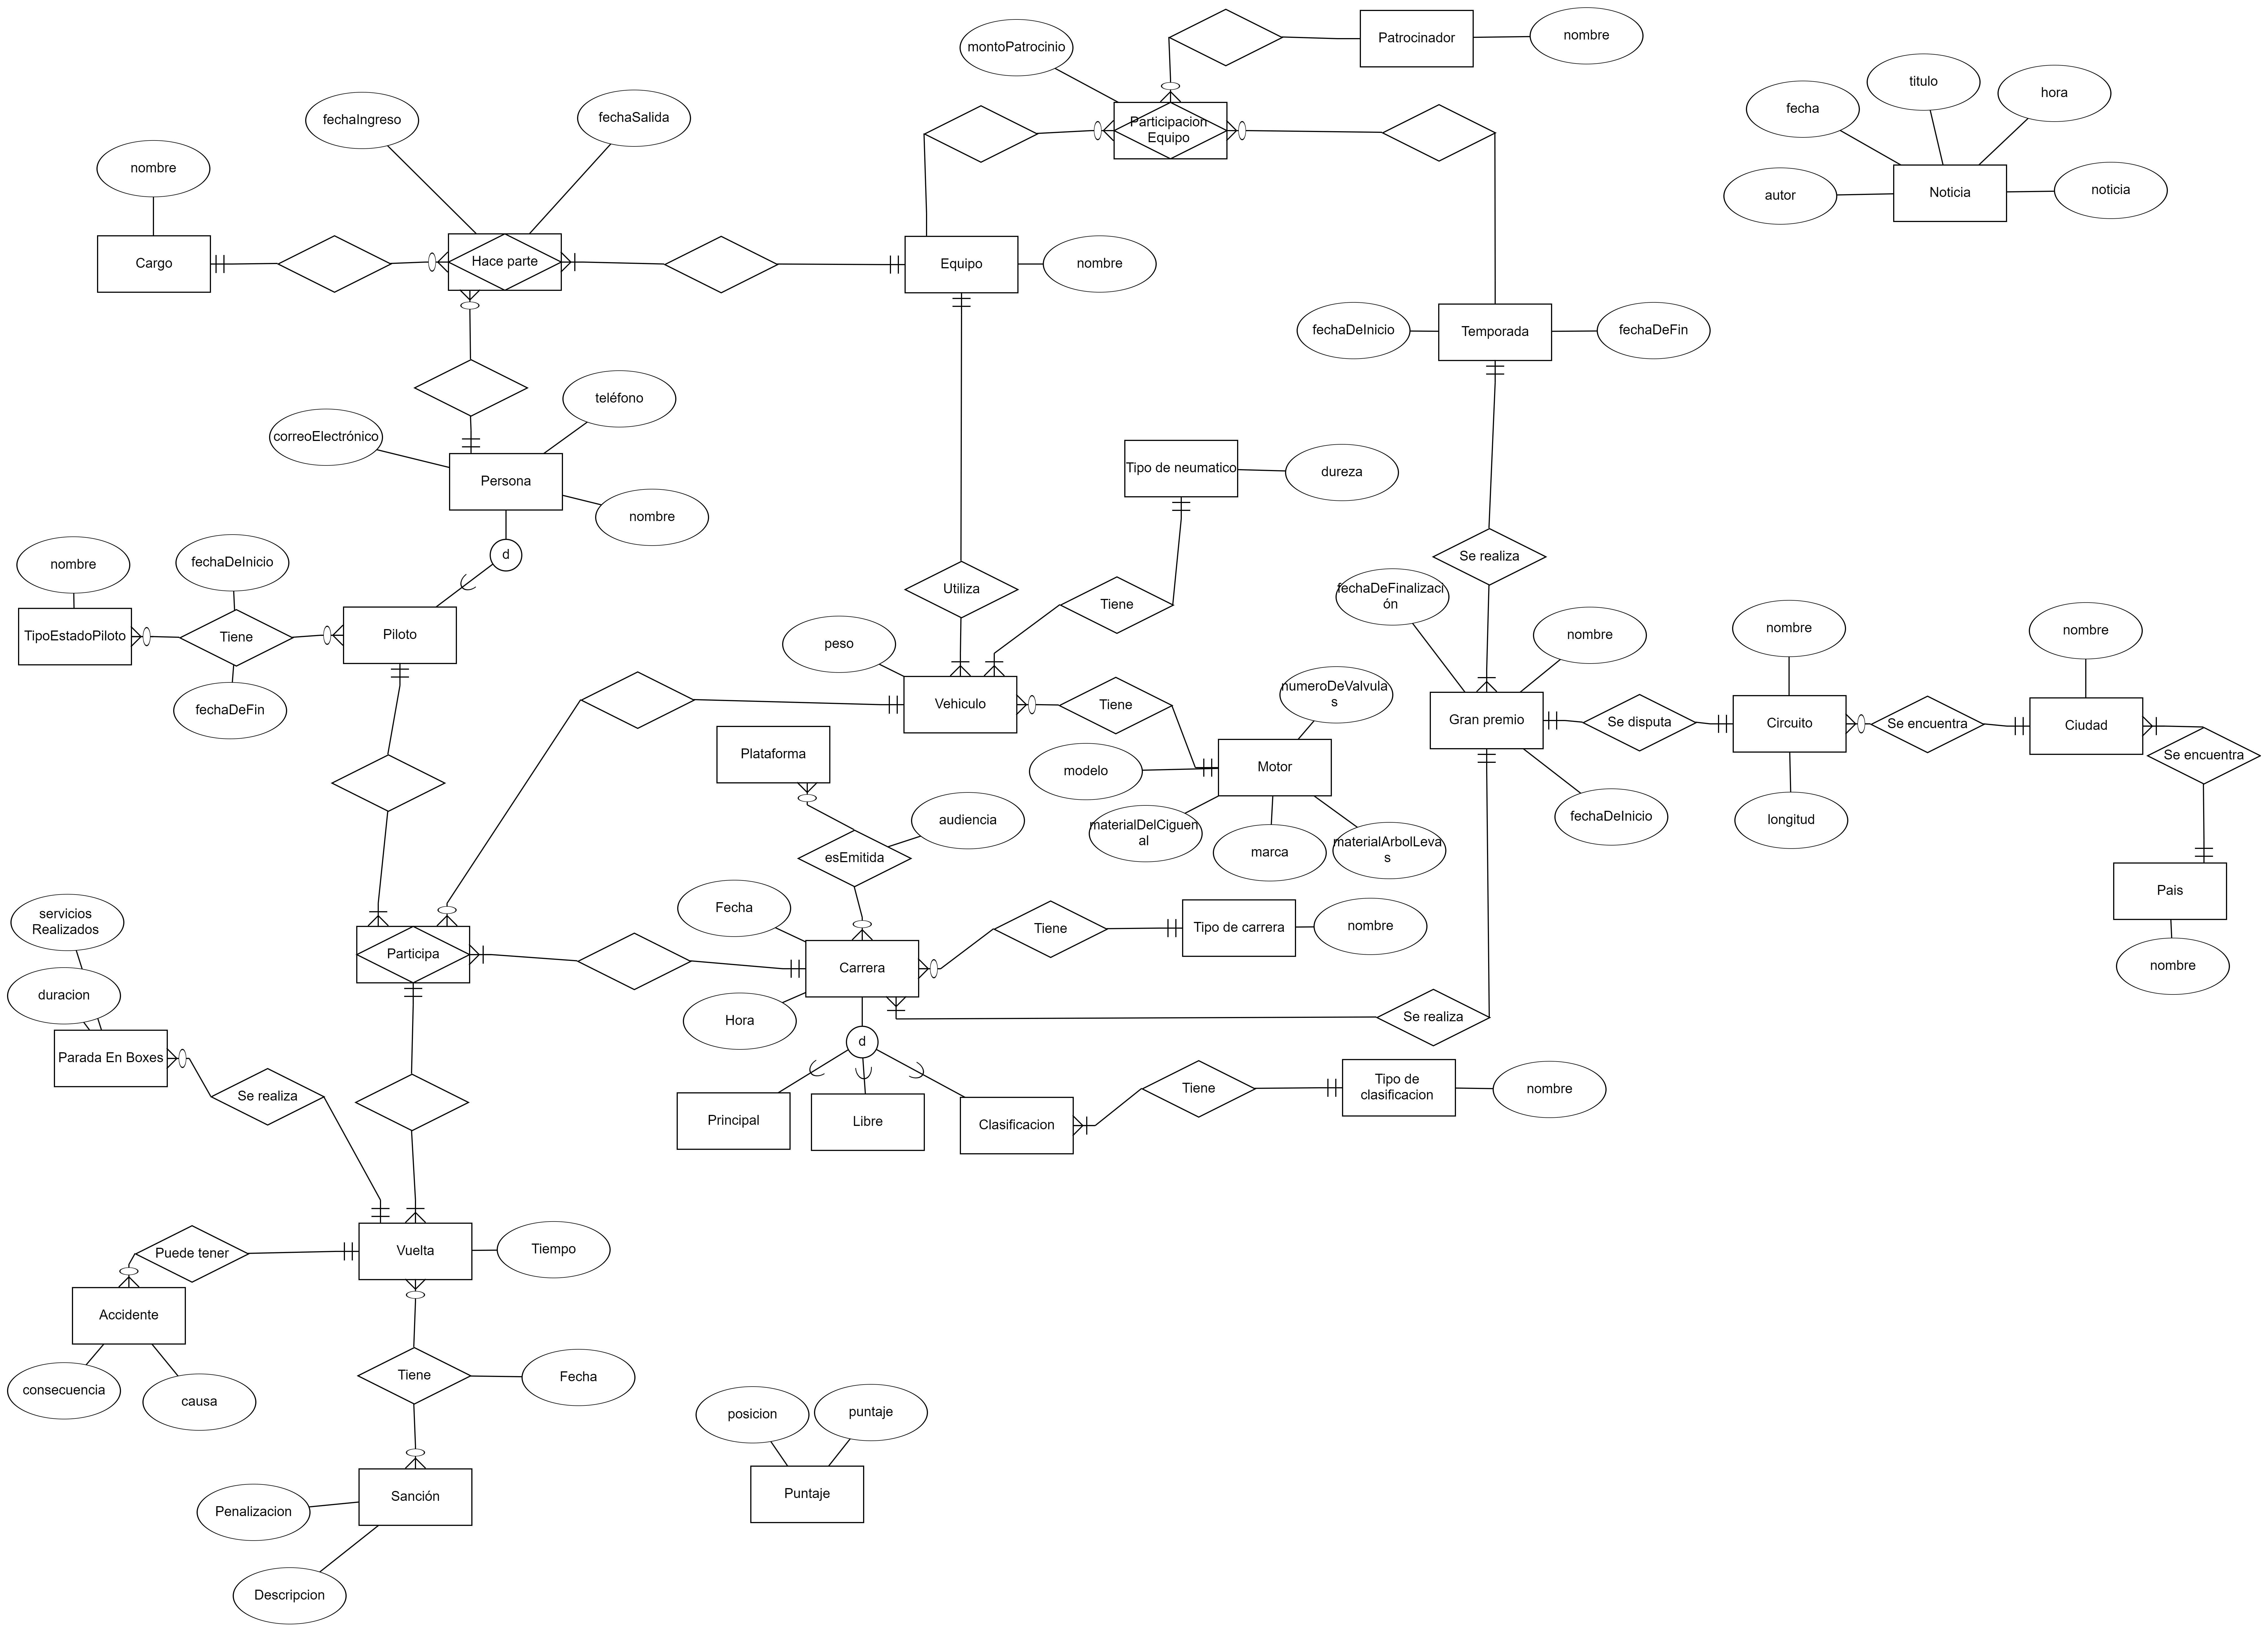
\includegraphics[width=\textwidth]{f1_conceptual}
	
	\section{Modelo Lógico}
	
	\includegraphics[width=\textwidth]{f1_Logico}
	
	\section{Preguntas}
	\begin{enumerate}
		\item ¿Cuál es el nombre y el país de las competiciones que se dieron en una temporada específica?
		\item ¿Cuál es el nombre del circuito más extenso que se utilizó en la temporada 4?
		\item ¿Cuáles son los circuitos aptos para realizar carreras fórmula 1?
		\item ¿Cuál es la marca, el tipo de neumáticos y el peso del vehículo del competidor X?
		\item ¿Cual es la posición, nombre del piloto, nacionalidad , el modelo de vehículo y los puntos que tienen los pilotos que participan en una temporada? Ordénelos por posición.
		\item ¿Cuál es el nombre, número de integrantes y el nombre del patrocinador de los equipos que participan en una temporada?
		\item ¿Cuál es el nombre, carrera y fecha de lesiones (si existe) que un piloto ha tenido en toda su trayectoria en la Fórmula 1?
		\item ¿Cuál es el nombre, la fecha y descripción de las sanciones que un piloto tuvo en una carrera determinada?
		\item ¿Cuál es la fecha, el país, la ciudad y el circuito de las carreras que ocurrirán próximamente? ordenadas por fecha
		\item ¿Cuál es el nombre, equipo y tiempo de un piloto determinado que ha participado en una carrera libre?
		\item ¿Cuál es el nombre del piloto, el número, la posición, el modelo del vehículo, el tiempo total en vueltas y el número de vueltas que hizo un piloto en una carrera?
		\item ¿Cuál es el nombre, apellido y cargo de los integrantes de un equipo determinado?
		\item ¿Cuál es el número de accidentes ocurridos en una temporada específica?
		\item ¿Cuál es el nombre del gran premio, la fecha, el modelo de vehículo, la posición y los puntos que hizo un piloto en una temporada?
		\item ¿Cuál es el fabricante y tipo de llanta más utilizado en una carrera determinada?
		\item ¿Cual es la posición, el nombre del equipo y los puntos que posee un equipo en una temporada en especifico? Ordenados por puntos.
		\item ¿Cuál es el nombre del gran premio, la fecha de fin y los puntos que ha tenido un equipo en una temporada?
		\item ¿Cuál es el nombre del equipo con más puntos en toda la historia de la Fórmula 1?
		\item ¿Cuál es el gran premio, el nombre del conductor, el vehículo y el tiempo de las vueltas más rápidas que se han hecho en cada gran premio de una temporada?
		\item ¿Cuál es el circuito que más se ha utilizado en toda la historia de la Fórmula 1?
		
	\end{enumerate}
	
	\section{Scripts SQL}
	\Large{\textbf{Consultas DDL (Data Definition Language)}} \par
	
	
		\textnormal{Accede al repositorio dando click \href{https://github.com/FaridBustos/FORMULA1/tree/main/DDL}{aqui}  o ingrensando el siguiente link "https://github.com/FaridBustos/FORMULA1/tree/main/DDL"}
	
	
	\Large{\textbf{Consultas DML (Data Manipulation Language)}} \par
	\textnormal{Accede al repositorio dando click \href{https://github.com/FaridBustos/FORMULA1/tree/main/DML}{aqui} o ingrensando el siguiente link "https://github.com/FaridBustos/FORMULA1/tree/main/DML"}
	
	
	

\end{document}
